\section{Experiments}

\begin{figure}[tb]
  \centering
  %
  \begin{subfigure}{0.31\linewidth}
  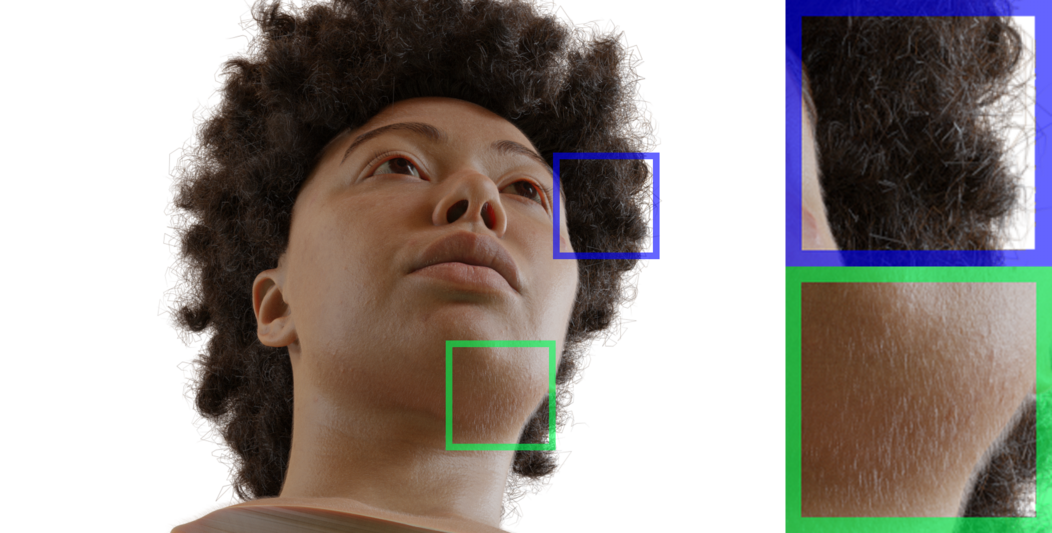
\includegraphics[width=\linewidth]{images/closeup/khady_gt_22_detail.png}
  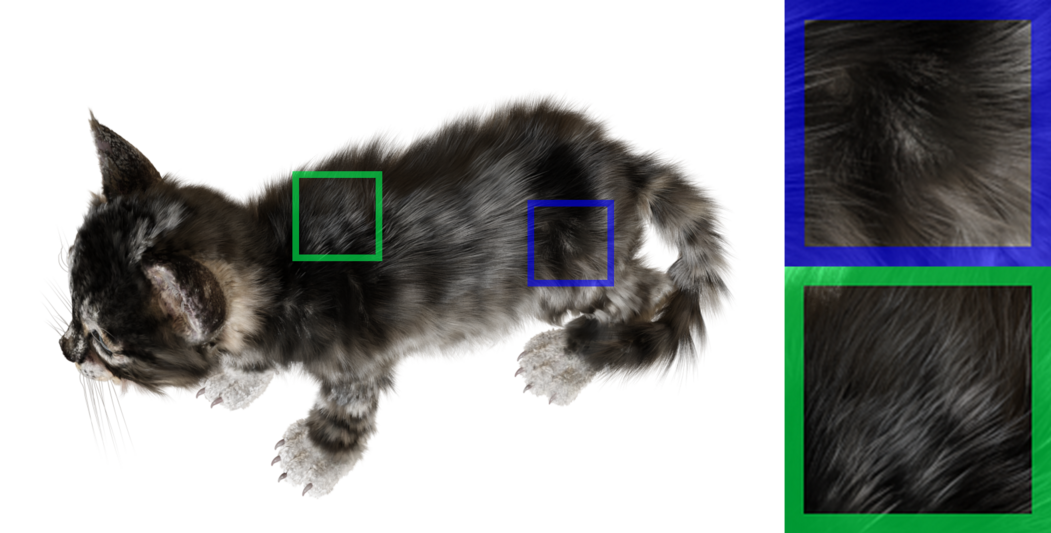
\includegraphics[width=\linewidth]{images/closeup/kitten_gt_67_detail.png}
  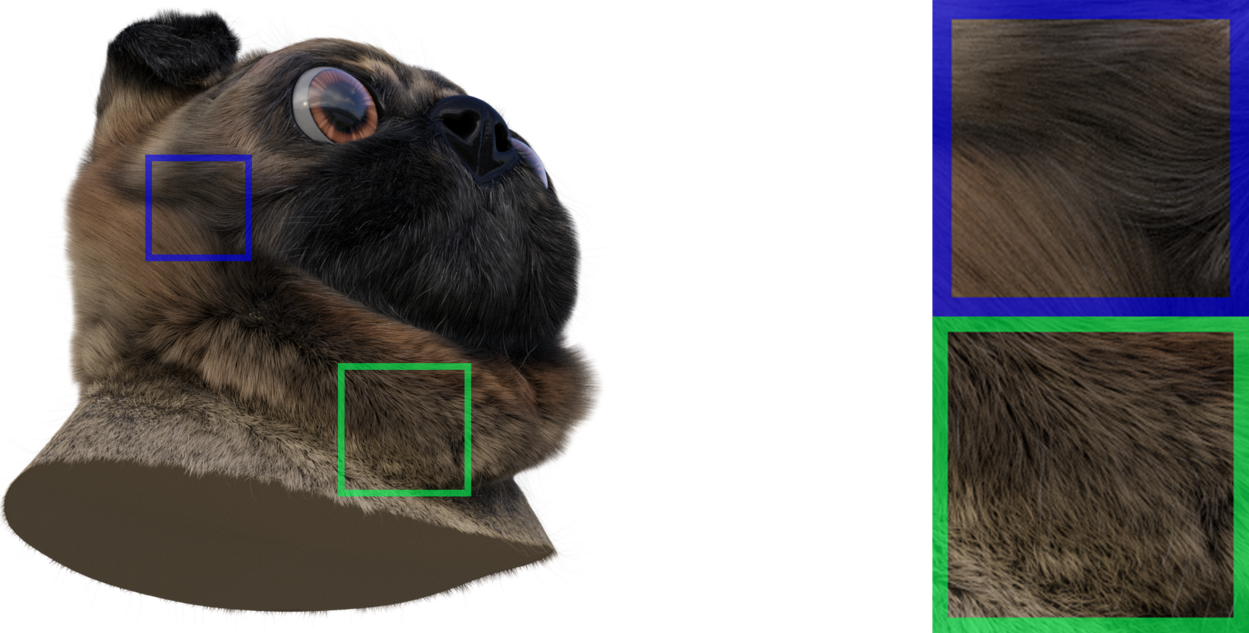
\includegraphics[width=\linewidth]{images/closeup/pug_gt_25_detail.png}
  \caption{Ground Truth Image}
  \end{subfigure}
  %
  \hfill
  %
  \begin{subfigure}{0.31\linewidth}
  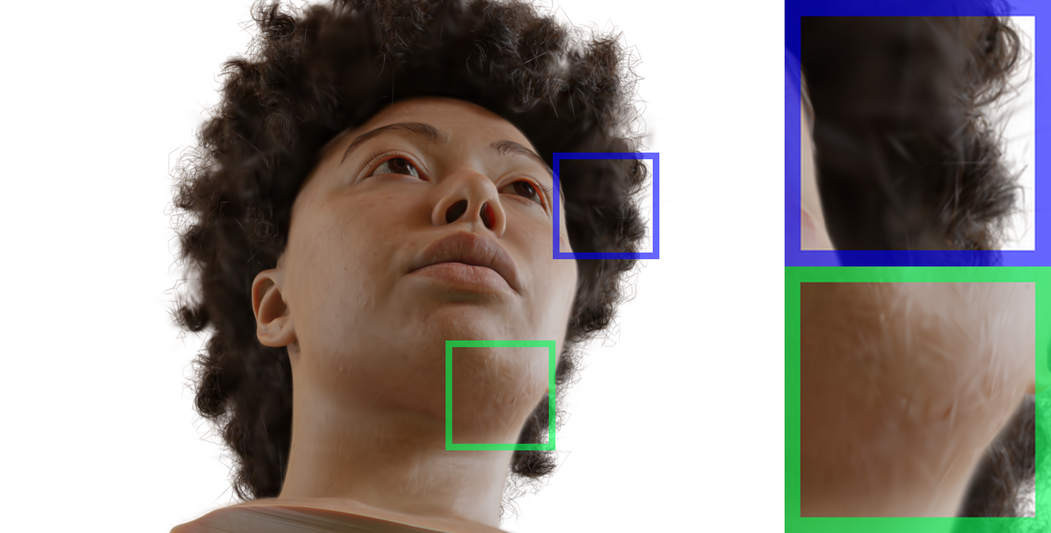
\includegraphics[width=\linewidth]{images/closeup/khady_3dgs_22_detail.png}
  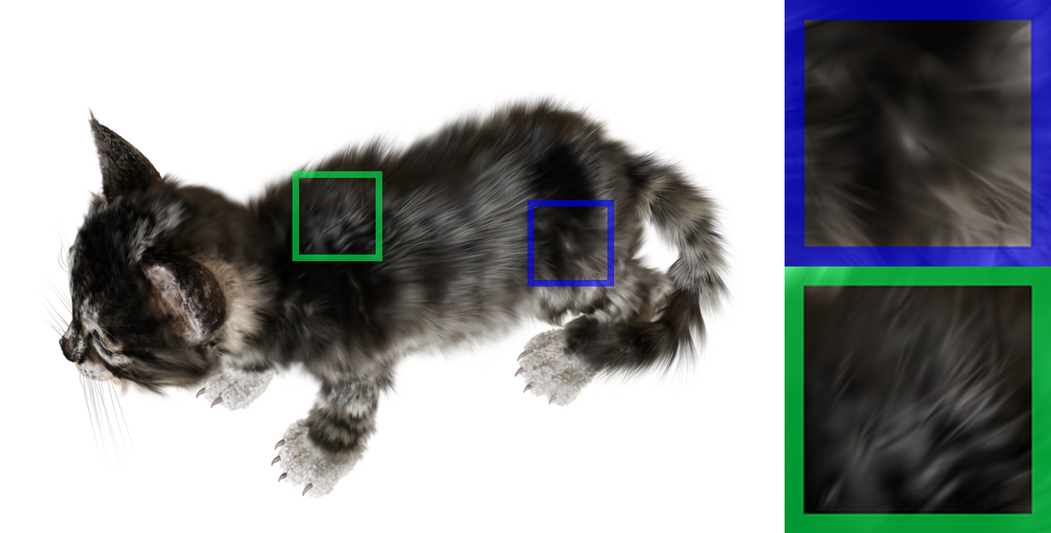
\includegraphics[width=\linewidth]{images/closeup/kitten_3dgs_67_detail.png}
  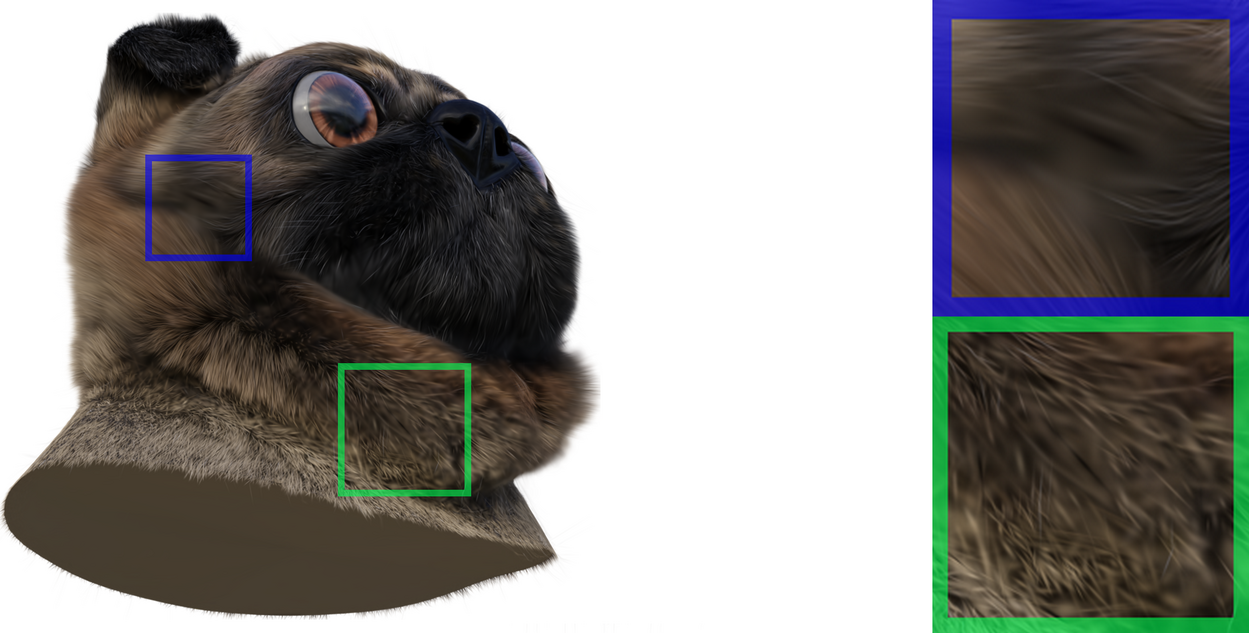
\includegraphics[width=\linewidth]{images/closeup/pug_3dgs_25_detail.png}
  \caption{3DGS~\cite{kerbl3Dgaussians}}
  \end{subfigure}
  %
  \hfill
  %
  \begin{subfigure}{0.31\linewidth}
  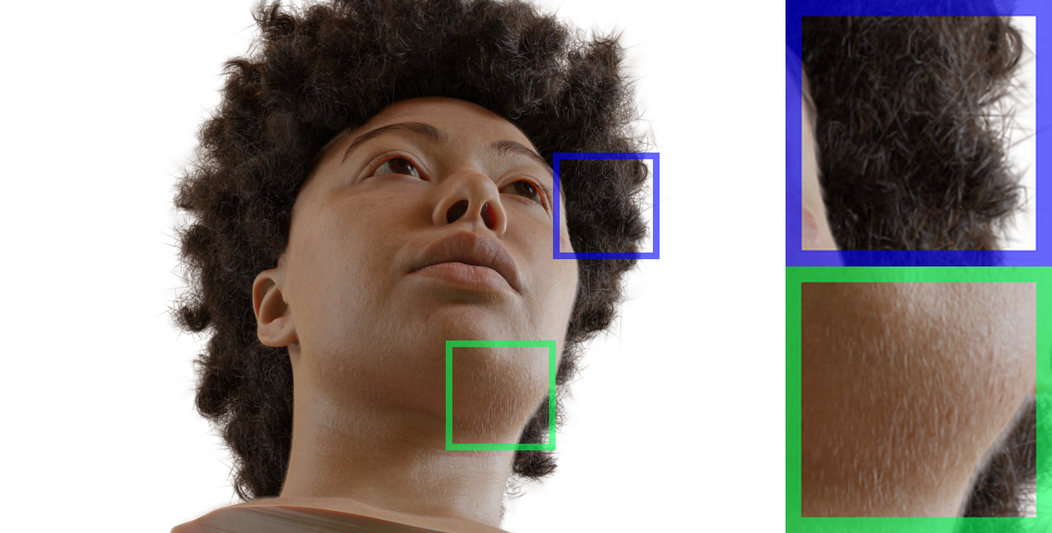
\includegraphics[width=\linewidth]{images/closeup/khady_rgb_22_detail.png}
  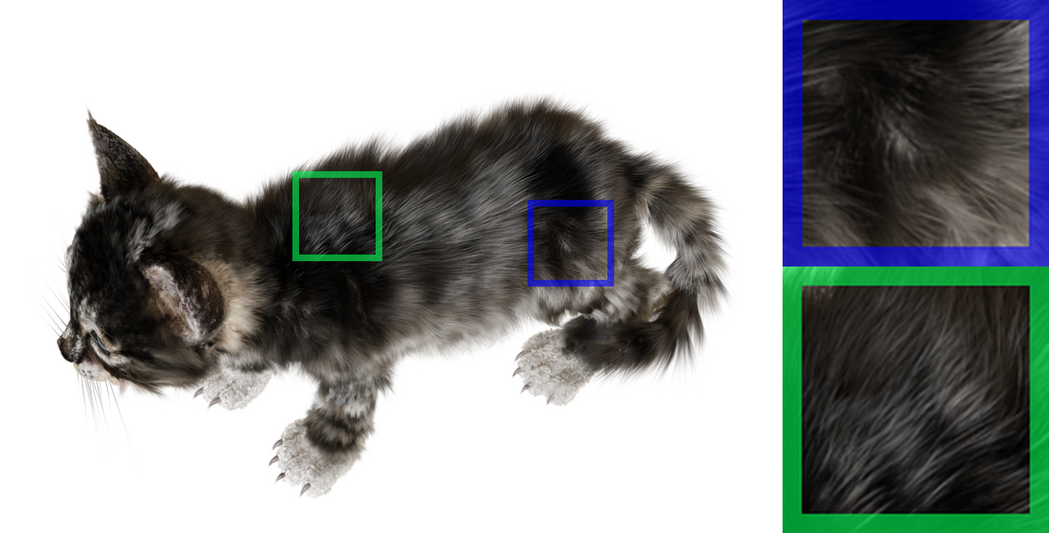
\includegraphics[width=\linewidth]{images/closeup/kitten_rgb_67_detail.png}
  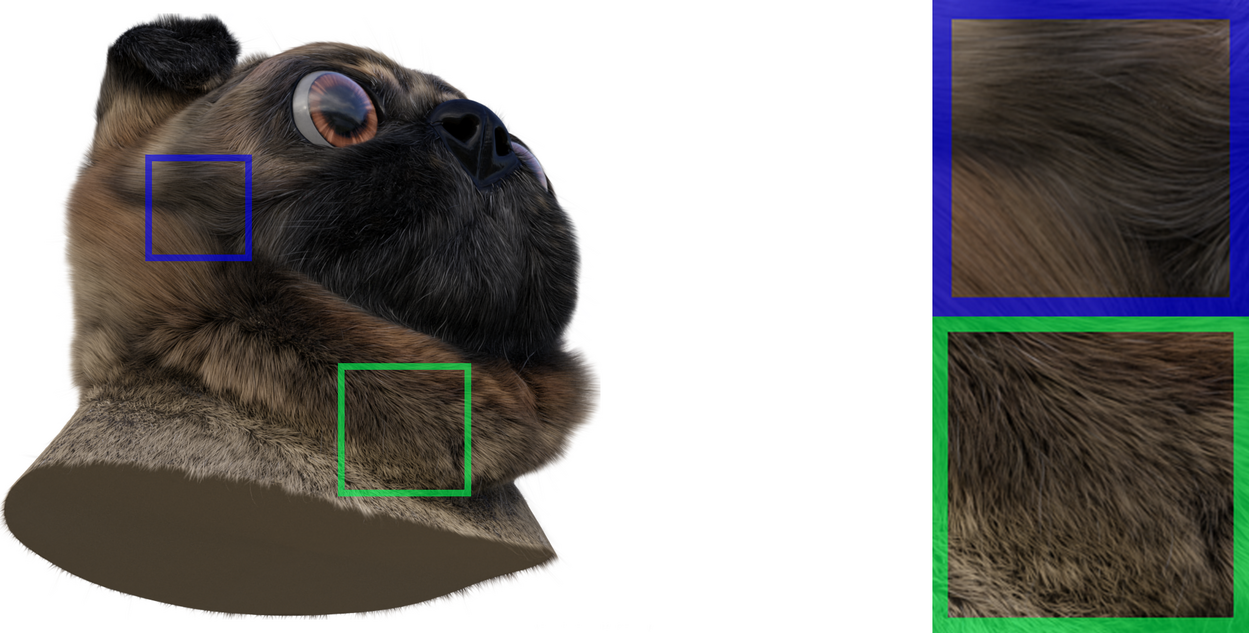
\includegraphics[width=\linewidth]{images/closeup/pug_rgb_25_detail.png}
  \caption*{Frosting (Ours)}
  \end{subfigure}
  %
  \vspace{-0.3cm}
  \caption{
  \textbf{Close-up views of fuzzy materials from the Shelly dataset~\cite{wang-siggraphasia2023-adaptive-shells} reconstructed with vanilla Gaussian Splatting~\cite{kerbl3Dgaussians}~(center) and Frosting~(right).}
  }
  \label{fig:fuzzy-material-closeup}
\end{figure}

\subsection{Implementation Details}


We implemented our method with PyTorch~\cite{paszke-nips19-pytorch} and optimized the representations on a single GPU Nvidia Tesla V100~SXM2~32~Go.
Optimizing a full, editable Frosting model takes between 45 and 90 minutes on a single GPU, depending on the complexity of the scene. This optimization is much faster than the most similar approach to Frosting in the literature, namely Adaptive~Shells~\cite{wang-siggraphasia2023-adaptive-shells}, that requires 8~hours on a single GPU for a synthetic scene, and 1.7 times more iterations for a real scene.

\subsubsection{Extracting the surface mesh.} When reconstructing real scenes, we follow the approach from vanilla 3DGS~\cite{kerbl3Dgaussians} and first use COLMAP to estimate the camera poses and extract a  point cloud for initialization. For synthetic scenes with known camera poses, we just use a random point cloud for initialization. Then, we optimize an unconstrained Gaussian Splatting representation for 7,000 iterations. We save these Gaussians aside and apply the regularization term from SuGaR until iteration~15,000. We finally compute an optimal depth parameter $\bar{D}$ with $\gamma=100$ and extract a mesh from the regularized Gaussians by applying Poisson surface reconstruction as described in~\cite{guedon2023sugar}.

\subsubsection{Optimizing the Gaussian Frosting.} Given a budget of $N$ Gaussians, we initialize $N$ Gaussians in the Frosting layer and optimize them for 15,000 additional iterations, which gives a total of 30,000 iterations, similarly to 3DGS~\cite{kerbl3Dgaussians}. Vanilla 3DGS optimization generally produces between 1 and 5 million Gaussians. In practice, we use $N$=5~million for real scenes and $N$=2~million for synthetic scenes.


\subsection{Real-Time Rendering in Complex Scenes}

To evaluate the quality of Frosting's rendering, we compute the standard metrics PSNR, SSIM and LPIPS~\cite{zhang-2018-cvpr-lpips} and compare to several baselines, some of them focusing only on Novel View Synthesis~\cite{mildenhall2020nerf,wang2021neus,barron2021mipnerf,barron2022mipnerf360,mueller2022instantngp,yu_and_fridovichkeil2021plenoxels,kerbl3Dgaussians} and others relying on an editable representation~\cite{chen2022mobilenerf,rakotosaona2023nerfmeshing,yariv-2023-bakedsdf,reiser2024binaryopacitygrid,wang-siggraphasia2023-adaptive-shells,guedon2023sugar}, just like Frosting. We compute metrics on several challenging datasets containing synthetic and real scenes.\\

\noindent
\textbf{Shelly.} We first compare Frosting to state-of-the-art methods on the dataset Shelly introduced in Adaptive~Shells~\cite{wang-siggraphasia2023-adaptive-shells}. Shelly includes six synthetic scenes with challenging fuzzy materials that surface-based approaches struggle to reconstruct accurately. As we show in Table~\ref{tab:nvsmetrics_shelly} and Figure~\ref{fig:fuzzy-material-closeup}, Frosting outperforms every other methods for all three metrics. Frosting even outperforms with a wide margin vanilla Gaussian Splatting, which is free from any surface constraints and only focuses on optimizing the rendering quality. Indeed, the sampling of Gaussians inside the Frosting layer provides a much more efficient densification of Gaussians than the strategy proposed in 3DGS~\cite{kerbl3Dgaussians}, targeting the challenging fuzzy areas close to the surface and allocating more Gaussians where volumetric rendering is needed.\\

\noindent
\textbf{NeRFSynthetic.} Table~\ref{tab:nvsmetrics_shelly} provides a comparison on the NeRFSynthetic data\-set~\cite{mildenhall2020nerf}, which consists in eight synthetic scenes. Frosting performs the best among the editable methods, surpassing Su\-GaR~\cite{guedon2023sugar}, and achieves results on par with vanilla 3DGS and other radiance field methods.\\

\begin{table}
   \caption{
   \antoine{
   \textbf{Quantitative evaluation of rendering quality on the synthetic datasets \emph{Shelly}~\cite{wang-siggraphasia2023-adaptive-shells} and \emph{NeRFSynthetic}~\cite{mildenhall2020nerf}.} Frosting is the best among all methods, outperforming even non-editable models that only focus on rendering. Contrary to an unconstrained 3D Gaussian Splatting~\cite{kerbl3Dgaussians}, our representation allows for densifying Gaussians more efficiently by targeting challenging and fuzzy areas.}}
  \label{tab:nvsmetrics_shelly}
  \centering
  {\scriptsize
  \begin{tabular}{@{}lccccccc@{}}
    \toprule
     \multicolumn{1}{c}{} & \multicolumn{3}{c}{\emph{Shelly}} & \multicolumn{3}{c}{\emph{NeRFSynthetic}} \\
     \cmidrule(r){2-4} \cmidrule(r){5-7}
      & PSNR $\uparrow$ & SSIM $\uparrow$ & LPIPS $\downarrow$ & PSNR $\uparrow$ & SSIM $\uparrow$ & LPIPS $\downarrow$ & \\
     %
    %\midrule
    %\multicolumn{4}{l}{\textbf{No mesh (except Frosting)}} \\
    \midrule
    NeRF~\cite{mildenhall2020nerf} & 31.27 & 0.893 & 0.157 & 31.01 & 0.947 & 0.081 & \\
    NeuS~\cite{wang2021neus} & 29.98 & 0.893 & 0.158 & -- & -- & -- & \\
    Mip-NeRF~\cite{barron2021mipnerf}  & 32.59 & 0.899 & 0.148 & \cellcolor{yellow!25}33.09 & 0.961 & 0.043 & \\
    I-NGP~\cite{mueller2022instantngp} & 33.22 & 0.922 & 0.125 & \cellcolor{orange!25}33.18 & -- & -- & \\
    3DGS~\cite{kerbl3Dgaussians}  & \cellcolor{orange!25}37.66 & \cellcolor{orange!25}0.958 & \cellcolor{orange!25}0.066 & \cellcolor{red!25}\textbf{33.32} & \cellcolor{red!25}\textbf{0.970} & \cellcolor{orange!25}0.030 & \\
    \midrule
    MobileNeRF~\cite{chen2022mobilenerf} & 31.62 & 0.911 & 0.129 & 30.90 & 0.947 & 0.062 & \\
    Adaptive Shells~\cite{wang-siggraphasia2023-adaptive-shells}  & 36.02 & \cellcolor{yellow!25}0.954 & 0.079 & 31.84 & 0.957 & 0.056 & \\
    SuGaR\cite{guedon2023sugar}  & \cellcolor{yellow!25}36.33 & \cellcolor{yellow!25}0.954 & \cellcolor{yellow!25}0.059 & 32.40 & \cellcolor{yellow!25}0.964 & \cellcolor{yellow!25}0.033 & \\
    Frosting (Ours)  & \cellcolor{red!25}\textbf{39.84} & \cellcolor{red!25}\textbf{0.977} & \cellcolor{red!25}\textbf{0.033} & 33.03 & \cellcolor{orange!25}0.967 & \cellcolor{red!25}\textbf{0.029} & \\
    \bottomrule
  \end{tabular}
  }
\end{table}

\noindent
\textbf{Mip-NeRF~360.} We also compare Frosting to state-of-the-art approaches on the real scenes from the Mip-NeRF~360 dataset~\cite{barron2022mipnerf360}. This dataset contains images from seven challenging real scenes, but was captured with ideal lighting condition and provides really good camera calibration data and initial SfM~points. Results are available in Table~\ref{tab:nvsmetrics_mipnerf360} and Figure~\ref{fig:frosting-renders}. Frosting reaches the best performance among all editable methods, and obtains worse but competitive results compared to vanilla Gaussian Splatting. When Gaussian Splatting is given a very good initialization with a large amount of SfM points, the benefits from the Gaussian Frosting densification are not as effective, and optimizing Gaussians without additional constraints as in 3DGS slightly improves performance.\\

\noindent
\textbf{Additional real scenes.} We finally compare Frosting to the baselines with captures of real scenes that present variations in exposure or white balance. To this end, we follow the approach from 3DGS~\cite{kerbl3Dgaussians} and select the same two subsets of two scenes from \emph{Tanks\&Temples} (\emph{Truck} and \emph{Train}) and \emph{Deep~Blending}~(\emph{Playroom} and \emph{Dr.~Johnson}). We also evaluate a few methods on a custom dataset that consists of four casual captures made with a smartphone (we call these scenes \emph{SleepyCat}, \emph{Buzz}, \emph{RedPanda}, and \emph{Knight}), illustrated in Figures~\ref{fig:teaser} and~\ref{fig:frosting-renders}. Results are available in Table~\ref{tab:nvsmetrics_tandtdb}. In these more realistic scenarios, Frosting achieves once again similar or better performance than unconstrained Gaussian Splatting even though it is an editable representation that relies on a single, animatable mesh.

\begin{table}
   \caption{\textbf{Quantitative evaluation of rendering quality on the Mip-NeRF~360 dataset~\cite{barron2022mipnerf360}.} \antoine{Frosting is best among the methods that recover an editable Radiance Field with explicit meshes, and achieves performance comparable to NeRF methods and vanilla 3D Gaussian Splatting.} }
  \label{tab:nvsmetrics_mipnerf360}
  \centering
  {\scriptsize
  \begin{tabular}{@{}lcccccccccc@{}}
    \toprule
      %
     \multicolumn{1}{c}{} & \multicolumn{3}{c}{Indoor scenes} & \multicolumn{3}{c}{Outdoor scenes} & \multicolumn{3}{c}{Average on all scenes} \\
     \cmidrule(r){2-4} \cmidrule(r){5-7} \cmidrule(r){8-10}
      & PSNR $\uparrow$ & SSIM $\uparrow$ & LPIPS $\downarrow$ & PSNR $\uparrow$ & SSIM $\uparrow$ & LPIPS $\downarrow$ & PSNR $\uparrow$ & SSIM $\uparrow$ & LPIPS $\downarrow$ \\
     %
    \midrule
    \multicolumn{10}{l}{\textbf{No mesh (except Frosting)}} \\
    \midrule
    Plenoxels~\cite{yu_and_fridovichkeil2021plenoxels} & 24.83 & 0.766 & 0.426 & 22.02 & 0.542 & 0.465 & 23.62 & 0.670 & 0.443 \\
    INGP-Base~\cite{mueller2022instantngp} & 28.65 & 0.840 & 0.281 & 23.47 & 0.571 & 0.416 & 26.43 & 0.725 & 0.339 \\
    INGP-Big~\cite{mueller2022instantngp} & 29.14 & 0.863 & 0.242 & 23.57 & 0.602 & 0.375 & 26.75 & 0.751 & 0.299 \\
    Mip-NeRF 360~\cite{barron2022mipnerf360} & \cellcolor{red!25}\textbf{31.58} & \cellcolor{yellow!25}0.914 & \cellcolor{red!25}\textbf{0.182} & \cellcolor{orange!25}25.79 & \cellcolor{yellow!25}0.746 & \cellcolor{yellow!25}0.247 & \cellcolor{red!25}\textbf{29.09} & \cellcolor{yellow!25}0.842 & \cellcolor{yellow!25}0.210 \\
    3DGS~\cite{kerbl3Dgaussians} & \cellcolor{yellow!25}30.41 & \cellcolor{orange!25}0.920 & \cellcolor{orange!25}0.189 & \cellcolor{red!25}\textbf{26.40} & \cellcolor{red!25}\textbf{0.805} & \cellcolor{red!25}\textbf{0.173} & \cellcolor{orange!25}28.69 & \cellcolor{red!25}\textbf{0.870} & \cellcolor{red!25}\textbf{0.182} \\
    Frosting (Ours) & \cellcolor{orange!25}30.49 & \cellcolor{red!25}\textbf{0.925} & \cellcolor{yellow!25}0.190 & \cellcolor{yellow!25}25.57 & \cellcolor{orange!25}0.765 & \cellcolor{orange!25}0.225 & \cellcolor{yellow!25}28.38 & \cellcolor{orange!25}0.856 & \cellcolor{orange!25}0.205\\
    \midrule
    \multicolumn{10}{l}{\textbf{With mesh}} \\
    \midrule
    MobileNeRF~\cite{chen2022mobilenerf} & 25.74 & 0.757 & 0.453 & 22.90 & 0.524 & 0.463 & 24.52 & 0.657 & 0.457 \\
    NeRFMeshing~\cite{rakotosaona2023nerfmeshing} & 23.83 & -- & -- & 22.23 & -- & -- & 23.15 & -- & -- \\
    BakedSDF~\cite{yariv-2023-bakedsdf} & 27.20 & 0.845 & 0.300 & \cellcolor{yellow!25}23.40 & 0.577 & \cellcolor{yellow!25}0.351 & 25.57 & 0.730 & \cellcolor{yellow!25}0.321 \\
    B.O. Grids~\cite{reiser2024binaryopacitygrid} & 27.71 & \cellcolor{yellow!25}0.873 & \cellcolor{yellow!25}0.227 & -- & -- & -- & -- & -- & -- \\
    Adaptive Shells~\cite{wang-siggraphasia2023-adaptive-shells} & \cellcolor{yellow!25}29.19 & 0.872 & 0.285 & 23.17  & \cellcolor{yellow!25}0.606 & 0.389 & \cellcolor{yellow!25}26.61 & \cellcolor{yellow!25}0.758 & 0.330 \\
    SuGaR\cite{guedon2023sugar} & \cellcolor{orange!25}29.43 & \cellcolor{orange!25}0.910 & \cellcolor{orange!25}0.216 & \cellcolor{orange!25}24.40 & \cellcolor{orange!25}0.699 & \cellcolor{orange!25}0.301 & \cellcolor{orange!25}27.27 & \cellcolor{orange!25}0.820 & \cellcolor{orange!25}0.253 \\
    Frosting (Ours) & \cellcolor{red!25}\textbf{30.49} & \cellcolor{red!25}\textbf{0.925} & \cellcolor{red!25}\textbf{0.190} & \cellcolor{red!25}\textbf{25.57} & \cellcolor{red!25}\textbf{0.765} & \cellcolor{red!25}\textbf{0.225} & \cellcolor{red!25}\textbf{28.38} & \cellcolor{red!25}\textbf{0.856} & \cellcolor{red!25}\textbf{0.205}\\
    \bottomrule
  \end{tabular}
  }
\end{table}
\begin{table}
   \caption{
   \antoine{
   \textbf{Quantitative evaluation of rendering quality on real scenes from \emph{Tanks\&Temples}~\cite{knapitsch-2017-tanksandtemples}, \emph{Deep~Blending}~\cite{hedman-2018-deepblending} and our custom dataset.} Our representation performs the best among the surface-based methods, and achieves similar or better performance than unconstrained 3DGS and other non-editable methods.}}
  \label{tab:nvsmetrics_tandtdb}
  \centering
  {\scriptsize
  \begin{tabular}{@{}lcccccccccc@{}}
    \toprule
     \multicolumn{1}{c}{} & \multicolumn{3}{c}{\emph{Tanks\&Temples}~\cite{knapitsch-2017-tanksandtemples}} & \multicolumn{3}{c}{\emph{Deep~Blending}~\cite{hedman-2018-deepblending}} & \multicolumn{3}{c}{\emph{Custom dataset}} \\
     \cmidrule(r){2-4} \cmidrule(r){5-7} \cmidrule(r){8-10}
      & PSNR $\uparrow$ & SSIM $\uparrow$ & LPIPS $\downarrow$ & PSNR $\uparrow$ & SSIM $\uparrow$ & LPIPS $\downarrow$ & PSNR $\uparrow$ & SSIM $\uparrow$ & LPIPS $\downarrow$ & \\
     %
    \midrule
    Plenoxels~\cite{yu_and_fridovichkeil2021plenoxels}  & 21.07 & 0.719 & 0.379 & 23.06 & 0.794 & 0.510 & -- & -- & -- &\\
    INGP-Base~\cite{mueller2022instantngp}  & 21.72 & 0.723 & 0.330 & 23.62 & 0.796 & 0.423 & -- & -- & -- & \\
    INGP-Big~\cite{mueller2022instantngp}  & 21.92 & 0.744 & 0.304 & 24.96 & 0.817 & 0.390 & -- & -- & -- & \\
    Mip-NeRF~360~\cite{barron2022mipnerf360}  & \cellcolor{yellow!25}22.22 & 0.758 & 0.257 & 29.40 & \cellcolor{orange!25}0.901 & \cellcolor{yellow!25}0.244 & -- & -- & -- & \\
    3DGS~\cite{kerbl3Dgaussians} & \cellcolor{red!25}23.14 & \cellcolor{red!25}0.841 & \cellcolor{orange!25}0.183 & \cellcolor{orange!25}29.41 & \cellcolor{red!25}0.903 & \cellcolor{orange!25}0.243 & \cellcolor{red!25}34.17 & \cellcolor{orange!25}0.944 & \cellcolor{orange!25}0.165 & \\
    \midrule
    SuGaR\cite{guedon2023sugar}  & 21.58 & \cellcolor{yellow!25}0.795 & \cellcolor{yellow!25}0.219 & \cellcolor{orange!25}29.41 & 0.893 & 0.267 & \cellcolor{yellow!25}32.05 & \cellcolor{yellow!25}0.930 & \cellcolor{yellow!25}0.180 & \\
    Frosting (Ours)  & \cellcolor{orange!25}23.13 & \cellcolor{orange!25}0.836 & \cellcolor{red!25}0.174 & \cellcolor{red!25}29.62 & \cellcolor{yellow!25}0.900 & \cellcolor{red!25}0.236 & \cellcolor{orange!25}33.82 & \cellcolor{red!25}0.945 & \cellcolor{red!25}0.149 & \\
    \bottomrule
  \end{tabular}
  }
\end{table}

\subsection{Editing, Compositing, and Animating Gaussian Frosting}

\begin{figure}[tb]
  \centering
  \begin{subfigure}{0.31\linewidth}
 %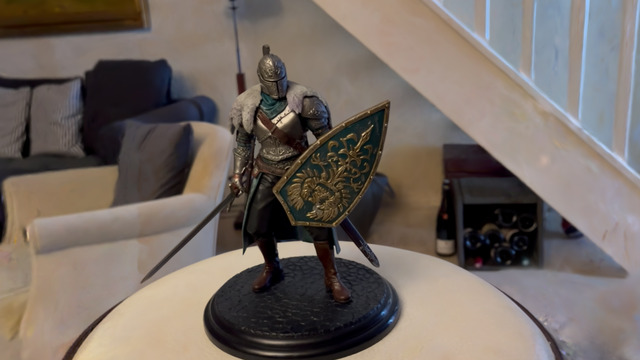
\includegraphics[trim={12cm 0 15cm 0},clip,width=\linewidth]{images/edition/faraam0_rgb_166.png}
 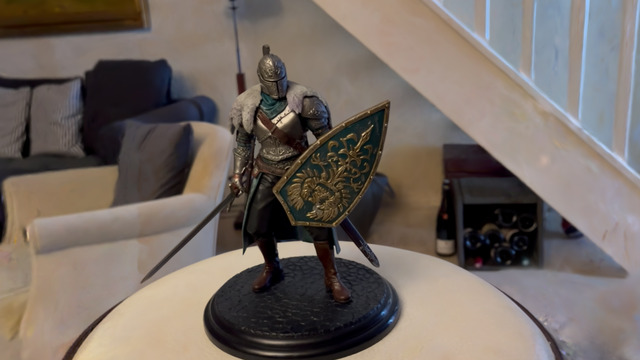
\includegraphics[trim={4cm 0 5cm 0},clip,width=\linewidth]{images/edition/faraam0_rgb_166.jpg}
 \caption{Original pose}
  \end{subfigure}
  %
  \hfill
  %
  \begin{subfigure}{0.31\linewidth}
  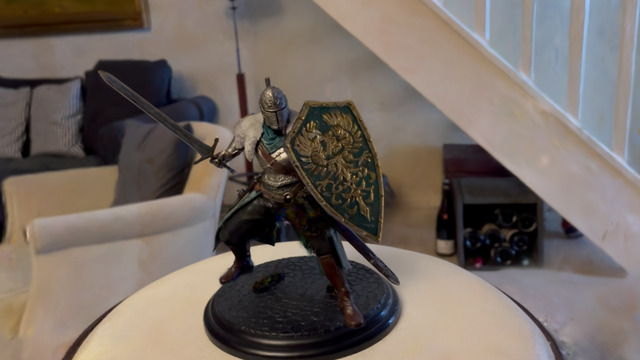
\includegraphics[trim={4cm 0 5cm 0},clip,width=\linewidth]{images/edition/faraam0_rgb_64.jpg}
  \caption{Edited pose}
  \end{subfigure}
  %
  \hfill
  \begin{subfigure}{0.31\linewidth}
  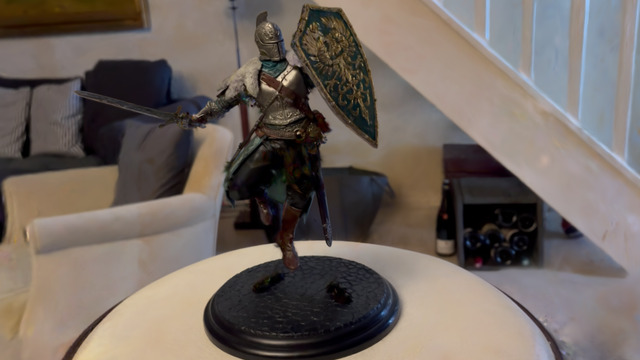
\includegraphics[trim={4cm 0 5cm 0},clip,width=\linewidth]{images/edition/faraam0_rgb_64_1.jpg}
  \caption{Edited pose}
  \end{subfigure}
  %
  \caption{
  \textbf{Examples of animation with Frosting.} We were able to animate the sculpture in the left image using the rigging tool in Blender.
  }
  \label{fig:edition-examples}
\end{figure}

As shown in Figure~\ref{fig:sugar-comparison}, Figure~\ref{fig:scene-composition} and Figure~\ref{fig:edition-examples}, our Frosting representation automatically adapts when editing, rescaling, deforming, combining or animating base meshes.
Frosting offers editing, composition and animation capabilities similar to surface-based approaches like SuGaR~\cite{guedon2023sugar}, but achieves much better performance thanks to its frosting layer with variable thickness that adapts to the volumetric effects and fuzzy materials in the scene.


\subsection{Ablation Study: Octree Depth}
\begin{table}
   \caption{
   \textbf{Ablation for two different depth computation methods used for the octree in Poisson surface reconstruction.} We compare the rendering performance between using a predefined depth with a high value as in~\cite{guedon2023sugar} and our automatically computed depth. Our technique systematically selects an optimal depth depending on the complexity of the scene, avoiding artifacts in the mesh, and resulting in equivalent or better rendering performance with a much smaller average number of triangles.
   }
  \label{tab:ablation-octree-depth}
  \centering
  {\scriptsize
  \begin{tabular}{@{}lccccccccc@{}}
    \toprule
     \multicolumn{1}{c}{} & \multicolumn{4}{c}{\emph{NeRFSynthetic}} & \multicolumn{4}{c}{\emph{Shelly}} \\
     \cmidrule(r){2-5} \cmidrule(r){6-9}
      & PSNR $\uparrow$ & SSIM $\uparrow$ & LPIPS $\downarrow$ & $N_{tri}$ $\downarrow$  & PSNR $\uparrow$ & SSIM $\uparrow$ & LPIPS $\downarrow$ & $N_{tri}$ $\downarrow$ & \\
     %
    \midrule
    Predefined depth $D$ = 10~\cite{guedon2023sugar} & 31.63 & 0.959 & 0.041 & >1 M & \cellcolor{red!25}\textbf{39.85} & 0.975 & 0.035 & 939 K &\\
    Depth $\bar{D} \leq 10$ & \cellcolor{red!25}\textbf{33.03} & \cellcolor{red!25}\textbf{0.967} & \cellcolor{red!25}\textbf{0.029} & \cellcolor{red!25}\textbf{863 K} & 39.84 & \cellcolor{red!25}\textbf{0.977} & \cellcolor{red!25}\textbf{0.033} & \cellcolor{red!25}\textbf{203 K} &\\
    \bottomrule
  \end{tabular}
  }
\end{table}

To demonstrate how our technique for automatically computing the optimal octree depth $\bar{D}$ for Poisson reconstruction improves the performance of Frosting, we provide in Table~\ref{tab:ablation-octree-depth} a comparison in rendering performance between our full model, and a version of Frosting that uses the same predefined depth parameter as SuGaR. This technique results in equivalent or better rendering performance with much fewer triangles.


\subsection{Ablation Study: Thickness of the Frosting Layer}
\begin{table}
   \caption{
   \textbf{Comparing different strategies for computing the thickness of the Frosting layer.} We compare the rendering performance (PSNR $\uparrow$) in synthetic and real scenes depending on how we compute and refine the thickness of the Frosting layer. Specifically, we first show that using an adaptive thickness improves performance over a constant thickness. Even though using a large constant thickness improves performance in scenes with very fuzzy materials like Shelly~\cite{wang-siggraphasia2023-adaptive-shells}, this lowers performance in scenes with flat surfaces and generates artifacts when editing the scene, as shown in Figure~\ref{fig:artifacts}. By contrast, our method adapts automatically to the type of surfaces. We also demonstrate that refining the thickness using the unconstrained Gaussians is necessary to achieve top performance.}
  \label{tab:ablation-proposal-intervals}
  \centering
  {\scriptsize
  \begin{tabular}{@{}lccccc@{}}
    \toprule
     \multicolumn{1}{c}{} & \multicolumn{1}{c}{\emph{\> Shelly \>}} & \multicolumn{3}{c}{\emph{Mip-NeRF~360}} \\
    \cmidrule(r){2-2} \cmidrule(r){3-5}
     & Average & Indoor & Outdoor & Average & \\
     %
    %\midrule
    %\multicolumn{4}{l}{\textbf{No mesh (except Frosting)}} \\
    \midrule
    Constant thickness (Small)  & 39.03 & \cellcolor{yellow!25}30.36 & 25.50 & \cellcolor{yellow!25}28.28 &  \\
    Constant thickness (Medium)  & \cellcolor{yellow!25}39.67 & 30.19 & \cellcolor{yellow!25}25.54 & 28.20 &  \\
    Constant thickness (Large) & \cellcolor{red!25}\textbf{40.00} & 30.06 & 25.48 & 28.10 &\\
    Using Regularized Gaussians only ($\delta^{\text{in/out}}=\epsilon^{\text{in/out}}$) & 39.34 & \cellcolor{orange!25}30.42 & \cellcolor{red!25}\textbf{25.57} & \cellcolor{orange!25}28.34 &  \\
     Using Regularized and Unconstrained Gaussians (Full method)  & \cellcolor{orange!25}39.84 & \cellcolor{red!25}\textbf{30.49} & \cellcolor{red!25}\textbf{25.57} & \cellcolor{red!25}\textbf{28.38} & \\
    \bottomrule
  \end{tabular}
  }
\end{table}
\begin{figure}[tb]
  \centering
  \begin{subfigure}{0.31\linewidth}
 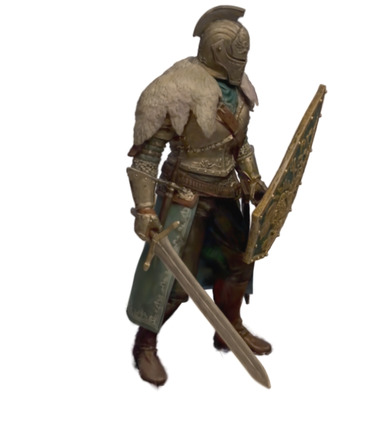
\includegraphics[width=\linewidth]{images/artifacts/static.jpg}
 \caption{\tiny Original pose}
  \end{subfigure}
  \hfill
  \begin{subfigure}{0.31\linewidth}
  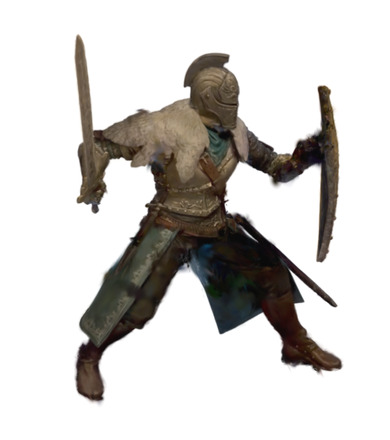
\includegraphics[width=\linewidth]{images/artifacts/no_artifact.jpg}
  \caption{\tiny Adaptive thickness (ours)}
  \end{subfigure}
  \hfill
  \begin{subfigure}{0.31\linewidth}
  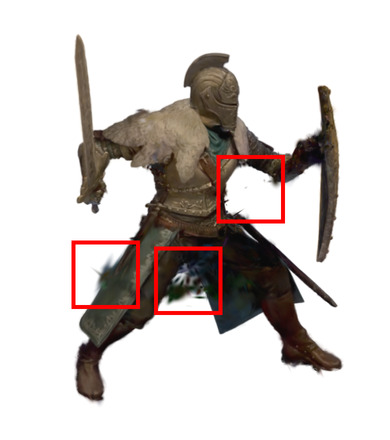
\includegraphics[width=\linewidth]{images/artifacts/with_artifact_0.jpg}
  \caption{\tiny Constant thickness (baseline)}
  \end{subfigure}
  %
  \caption{
  \textbf{Comparison with a constant thickness.} Our strategy to compute an adaptive thickness for Frosting is essential to maintain optimal performance while avoiding artifacts when editing the scene. As shown in the right image, using a constant thickness may produce artifacts when animating a character: When using a constant, large thickness in this scene, Gaussians located near the right knee of the knight participate in reconstructing the right hand, which produces artifacts when moving the hand.
  }
  \label{fig:artifacts}
\end{figure}

We also provide in Table~\ref{tab:ablation-proposal-intervals} an ablation study comparing different strategies for computing the thickness of the Frosting layer. 
%
Specifically, we first evaluate the rendering performance of a Frosting layer with constant thickness. We repeat the experiment for small, medium and large thickness values, using different quantiles of our inner and outer shifts~$\innershift$ and $\outershift$ for computing the constant thickness.
%
We show that using an adaptive thickness improves performance over a constant thickness, as (a) some fuzzy materials need a thicker frosting to be accurately rendered, and (b) some flat surfaces are better rendered with a very thin frosting. 
%
As a consequence, even though using a large constant thickness improves performance in scenes with very fuzzy materials like Shelly~\cite{wang-siggraphasia2023-adaptive-shells}, it lowers performance in scenes with flat surfaces. Moreover, using an adaptive thickness rather than a constant thickness with a large value helps to greatly reduce artifacts, as we demonstrate in Figure~\ref{fig:artifacts}.

We also show that using unconstrained Gaussians to refine the thickness of the Frosting is necessary to achieve top performance. To this end, we skip the refinement process and evaluate the rendering performance of a Frosting layer with $\innershift=\propinnershift$ and $\outershift=\propoutershift$. This results in lower performance, as shown in Table~\ref{tab:ablation-proposal-intervals}.